% kompilace xelatex prezentace.tex
% dokumentace k beameru: http://ftp.cvut.cz/tex-archive/macros/latex/contrib/beamer/doc/beameruserguide.pdf

% nastavení formátu prezentace 16:9
\documentclass[czech,aspectratio=169]{beamer}

\usepackage{polyglossia}
\setmainlanguage{czech}

% nastavení vzhledu
% další možnosti vzhledu viz https://hartwork.org/beamer-theme-matrix/
\usetheme{Madrid}
\usecolortheme{whale}
\usepackage{subfig}

\usepackage{amsmath}
\usepackage{amsfonts}


\usepackage{tikz}
\usetikzlibrary{fadings}
\newcommand{\gradient}{\noindent%
	\begin{tikzpicture}
		\fill[black,path fading=west] (-0.5\linewidth,0) rectangle (0,1ex);
		\fill[black,path fading=east] (0,0) rectangle (0.5\linewidth,1ex);
	\end{tikzpicture}%
}

% for setting different borders
\usepackage{geometry}

% left, right v includegraphics
\usepackage[export]{adjustbox}

\usepackage{media9}
\usepackage{graphicx} % prehravani videa

%\usepackage[shortlabels]{enumitem}
\usepackage{enumerate}
%\usepackage{enumitem}

% vzhled slajdů vnitřní téma (např. vzhled odrážek)
\useinnertheme{rectangles} %možnosti: default circles rectangles rounded inmargin
% vzhled slajdů vnější téma
\useoutertheme{default} %možnosti: default, miniframes, smoothbars, sidebar, split, shadow, tree, smoothtree, infolines

% zavedeme čvutí modou barvu
\definecolor{CVUT}{HTML}{0065BD}
% čvutí modou použijeme jako hlavní barvu prezentace
\setbeamercolor{structure}{bg=white,fg=CVUT}

% jako font prezentace nadefinujeme oficiální ČVUT písmo Technika -- pokud chcete použít, musíte si font nainstalovat nebo jej nahrát na Overleaf
% https://www.cvut.cz/logo-a-graficky-manual  -- inforek, přihlášení přes celoškolské heslo
%\usepackage{fontspec}
%\setsansfont{Technika-Kniha}

% vypneme navigační panel beamer (pro zapnutí zakomentujeme)
\beamertemplatenavigationsymbolsempty

% vygenerujeme slajdy s poznámkami -- ty si můžete vytisknout a mít je na obhajobu s sebou (pokud zapomenete slova, nebo kdyby nefungovalo promítání z nějakého důvodu)
%\setbeameroption{show notes}

% vygeneruje slajdy s poznámky vhodné pro promítání na dvou monitorech -- na obhajobu nevyužijete
%\usepackage{pgfpages}
%\setbeameroption{show notes on second screen}

% variable block width
\newenvironment<>{varblock}[2][.9\textwidth]{%
    \setlength{\textwidth}{#1}
        \begin{actionenv}
            #3%
            \def\insertblocktitle{#2}%
    \par%
    \usebeamertemplate{block begin}}
    {\par%
\usebeamertemplate{block end}%
\end{actionenv}}

\usepackage{graphicx}
\graphicspath{{../thesis/figures}}

% fromat datumu
\usepackage[style=dmyyyy,datesep={.}]{datetime2}

% další balíčky
\usepackage{graphicx}
\usepackage{minted}
\usepackage{hyperref}
\usepackage{tikz}
\usetikzlibrary{chains,fit,shapes}

\newcommand{\navesti}[1]{\noindent\textbf{\textit{{#1}}}}
\newcommand{\definice}[1]{\textbf{\textit{{#1}}}}
\DeclareMathOperator*{\argmax}{arg\,max}
\DeclareMathOperator*{\argmin}{arg\,min}
\DeclareMathOperator*{\real}{\mathbb{R}}
\DeclareMathOperator*{\realpos}{\mathbb{R}^+}
\DeclareMathOperator*{\nat}{\mathbb{N}}
\DeclareMathOperator*{\natpos}{\mathbb{N}^+}

% Údaje o prezentaci
\title[Optimalizace rozmístění obrazů]{Optimalizace rozmístění obrazů pomocí evolučních technik}
\subtitle{Magisterská práce}
\institute[FIT ČVUT v Praze]{Fakulta informačních technologií \\ České vysoké učení technické v Praze}
\author[M. Šafránek]{Bc.\,Martin Šafránek \\ Vedoucí práce: doc.\,RNDr\,Ing\,Marcel Jiřina,\,Ph.D.}
%\date{\today}
\date{}
\titlegraphic{
\includegraphics[width=.1\textwidth]{logo-cvut}}


\begin{document}

\begin{frame}
	\titlepage
	\note{Nezapomenout pozdravit} %tohle je poznámka, ta na slajdu nebude, ale vygeneruje se vedle něj, pokud odkomentujete příkaz výše -- \setbeameroption{show notes}
\end{frame}

%%%%%%%%%%%%%%%%%%%%%%%%%%%%%%%%%%%%%%%%%%%%%%%%%%%%%%%%%%%%%%%%%%%%%%%%%%%%%%
%%%%%%%%%%%%%%%%%%%%%%%%%%%%%%%%%%%%%%%%%%%%%%%%%%%%%%%%%%%%%%%%%%%%%%%%%%%%%%

\begin{frame}{Cíle práce}
	\begin{columns}
		\begin{column}{.5\textwidth}
			\begin{itemize}
				\item \textbf<2>{navrhnout a implementovat evoluční algoritmus pro rozmístění obrazů na stěně}
				\item \textbf<3>{vyhodnotit a vizualizovat výsledky}
				\item \textbf<4>{navrhnout zlepšení, rozšíření}
			\end{itemize}
		\end{column}
		\begin{column}{.5\textwidth}
			\includegraphics<3-4>[width=0.8\textheight]{london_gallery_wall}
		\end{column}
	\end{columns}
\end{frame}


%%%%%%%%%%%%%%%%%%%%%%%%%%%%%%%%%%%%%%%%%%%%%%%%%%%%%%%%%%%%%%%%%%%%%%%%%%%%%%
\section{Formulace problému}
%%%%%%%%%%%%%%%%%%%%%%%%%%%%%%%%%%%%%%%%%%%%%%%%%%%%%%%%%%%%%%%%%%%%%%%%%%%%%%

\begin{frame}{Formulace problému}

	\begin{columns}[T]

		\begin{column}{.3\textwidth}
			\centering
			\begin{enumerate}[a]
				\item vzájemný vztah mezi jednotlivými obrazy
				\item vztah obrazů a umístění na stěně
				\item penalizace za špatné umístění
			\end{enumerate}
		\end{column}

		\begin{column}{.5\textwidth}
			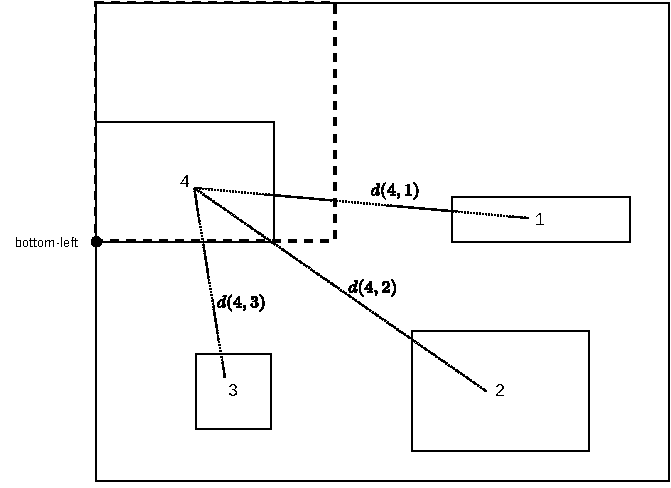
\includegraphics[width=0.75\textheight]{corner_placing_heuristic}
		\end{column}
	\end{columns}

	\begin{equation}
		\argmin_{x \in S} c(x) =
		\underbrace{\sum\limits_{i=1}^N\sum\limits_{j=i+1}^N f_{i,j}d(i, j)}_{a} +
		\underbrace{\sum\limits_{i=1}^N \pi(i)}_{b} + \underbrace{\lambda m(x) + \gamma n(x)}_{c} \,,
		%			\label{eq:objective}
	\end{equation}
\end{frame}


%%%%%%%%%%%%%%%%%%%%%%%%%%%%%%%%%%%%%%%%%%%%%%%%%%%%%%%%%%%%%%%%%%%%%%%%%%%%%%
\section{Genetický algoritmus}
%%%%%%%%%%%%%%%%%%%%%%%%%%%%%%%%%%%%%%%%%%%%%%%%%%%%%%%%%%%%%%%%%%%%%%%%%%%%%%


\begin{frame}{Genetický algoritmus – princip fungování}
	\begin{columns}[T]
		\begin{column}{.5\textwidth}
			\centering
			\begin{itemize}
				\item inspirován přirozeným výběrem v přírodě
				\item randomizovaný iterativní algoritmus
				\item stěžejí části \begin{itemize}
					      \item kódování jedince
					      \item fitness
					      \item genetické operátory
					            \begin{itemize}
						            \item křížení, mutace, ...
					            \end{itemize}
					      \item reprodukční schéma
				      \end{itemize}
			\end{itemize}
		\end{column}

		\begin{column}{.5\textwidth}
			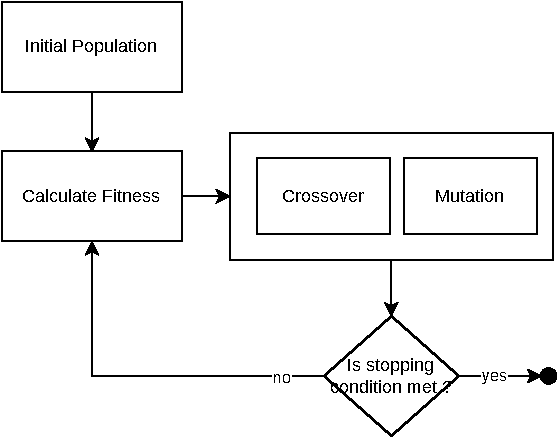
\includegraphics[width=0.8\textwidth]{reproductive_plan}
		\end{column}

	\end{columns}

\end{frame}

\begin{frame}{Genetický algoritmus – kódování jedince}
	\begin{columns}[T]
		\begin{column}{.5\textwidth}
			\centering
			\begin{itemize}
				\item dva stochastické vektory, jedna stochastická matice
				\item jedinec reprezentuje alespoň jedno rozmístění obrazů
			\end{itemize}
		\end{column}

		\begin{column}{.5\textwidth}
			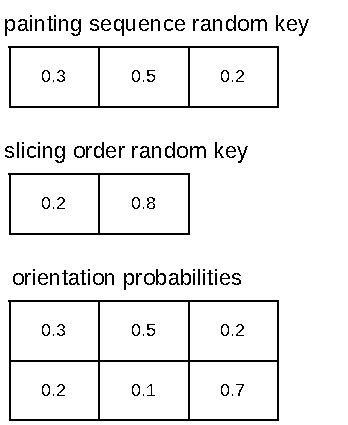
\includegraphics[width=0.6\textwidth]{./img/chromosome}
		\end{column}

	\end{columns}
\end{frame}

\begin{frame}{Genetický algoritmus – křížení}
	\begin{columns}[T]
		\begin{column}{.3\textwidth}
			\centering
			\begin{itemize}
				\item unikátní řešení
				\item aproximace rozdělení, které poskytuje dobré výsledky
				\item vždy vytvoří validního jedince
			\end{itemize}
		\end{column}
		\begin{column}{.5\textwidth}
			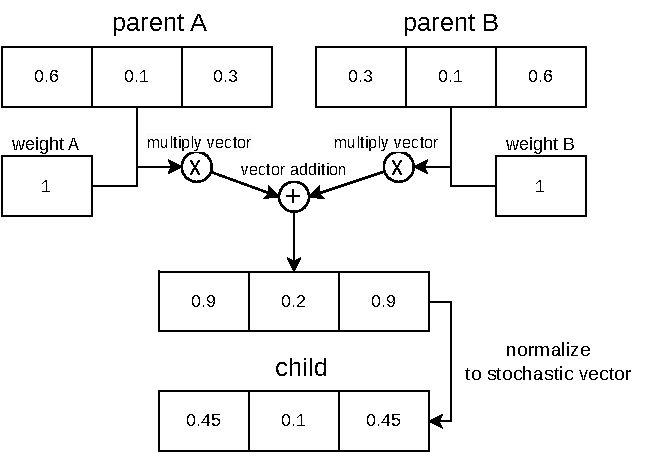
\includegraphics[width=1.0\textwidth]{./img/crossover-101}
		\end{column}
	\end{columns}

\end{frame}

\begin{frame}{Genetický algoritmus – dekódování jedince}
	\begin{columns}[T]
		\begin{column}{1.0\textwidth}
			\begin{itemize}
				\item náhodné klíče
				\item typ řezu s nejvyšší pravděpodobností – H, V nebo \textit{*}
				\item dekódovaný jedinec reprezentuje jeden řezový strom (slicing tree)
			\end{itemize}
		\end{column}

	\end{columns}
	\vfill \begin{figure}
		\centering
		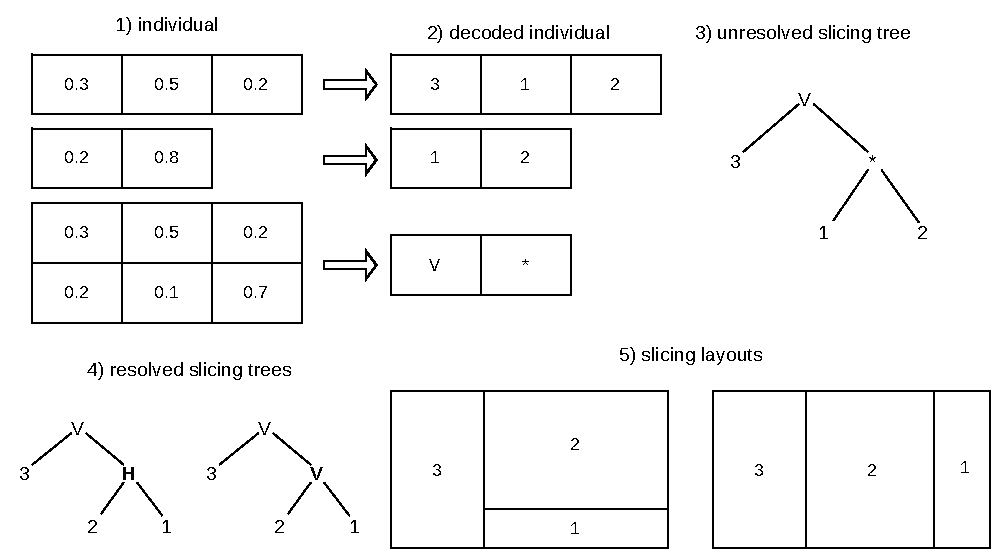
\includegraphics[width=0.7\textwidth]{./img/decoding-step}
	\end{figure}
\end{frame}

%%%%%%%%%%%%%%%%%%%%%%%%%%%%%%%%%%%%%%%%%%%%%%%%%%%%%%%%%%%%%%%%%%%%%%%%%%%%%%
\section{Konstrukce řešení}
%%%%%%%%%%%%%%%%%%%%%%%%%%%%%%%%%%%%%%%%%%%%%%%%%%%%%%%%%%%%%%%%%%%%%%%%%%%%%%

\begin{frame}{Konstrukce řešení 1/2 – slicing layout}
	\begin{columns}[T]
		\begin{column}{1.0\textwidth}
			\centering
			\begin{itemize}
				\item rozdělení stěny na části
				\item přiřazení každému obrazu jeho alokovaný prostor na stěne
				\item unikátní rozšíření typu řezu o symbol \textit{*}
			\end{itemize}
		\end{column}

		%		\begin{column}{.5\textwidth}
		%			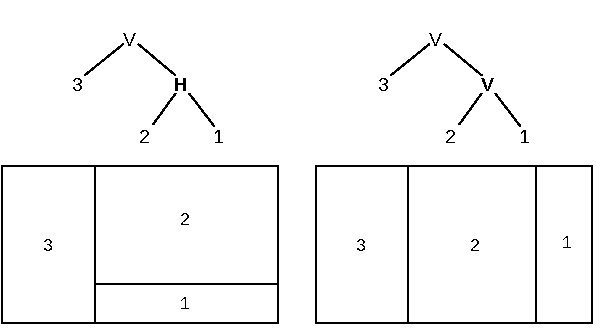
\includegraphics[width=0.75\textwidth]{./img/slicing-layout-101}
		%		\end{column}
	\end{columns}

	\vfill \begin{figure}
		\centering
		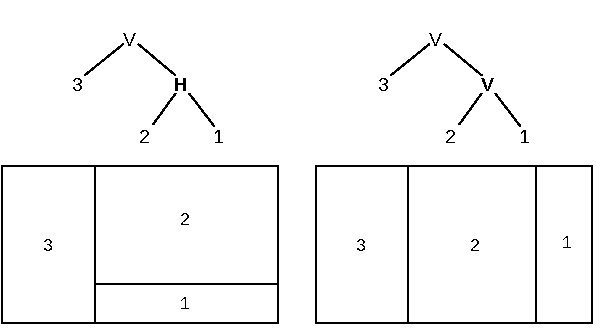
\includegraphics[width=0.65\textwidth]{./img/slicing-layout-101}
	\end{figure}
\end{frame}

\begin{frame}{Konstrukce řešení 2/2}
	\begin{columns}[T]
		\begin{column}{.5\textwidth}
			\centering
			\begin{itemize}
				\item iterativní greedy heuristika
				\item v každém kroku se snaží umístit jeden obraz tak, aby minimalizovala objektivní funkci
				\item pořadí umísťování je dáno pořadím po dekódování jedince
			\end{itemize}
		\end{column}

		\begin{column}{.5\textwidth}
			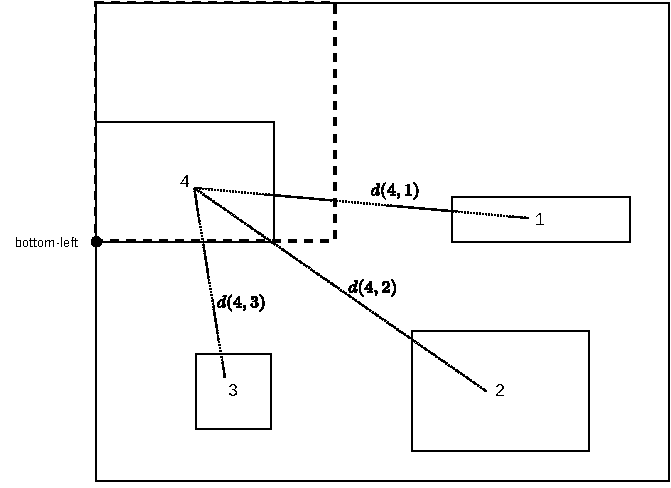
\includegraphics[width=0.95\textwidth]{corner_placing_heuristic}
		\end{column}
	\end{columns}
\end{frame}


%%%%%%%%%%%%%%%%%%%%%%%%%%%%%%%%%%%%%%%%%%%%%%%%%%%%%%%%%%%%%%%%%%%%%%%%%%%%%%
\section{Výsledky}
%%%%%%%%%%%%%%%%%%%%%%%%%%%%%%%%%%%%%%%%%%%%%%%%%%%%%%%%%%%%%%%%%%%%%%%%%%%%%%

\begin{frame}{Výsledky 1/2}
	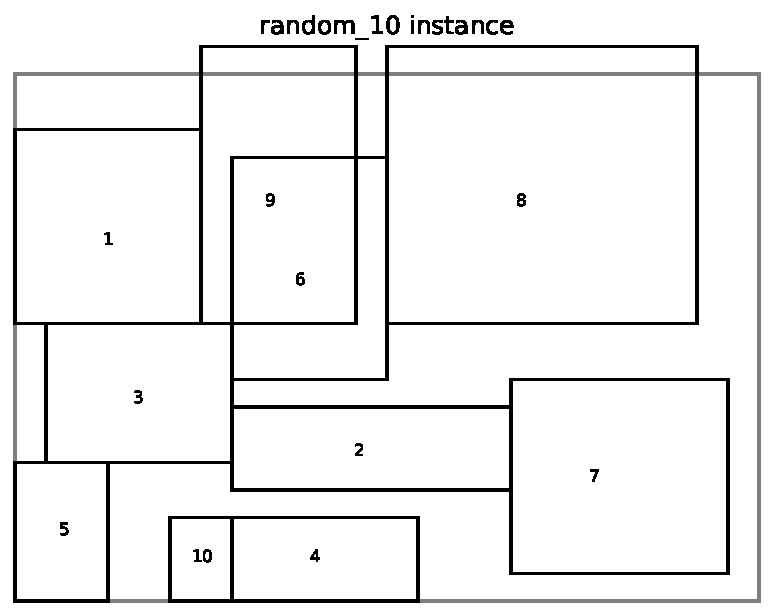
\includegraphics[width=0.49\textwidth]{visualizations/visualization_random_10}
	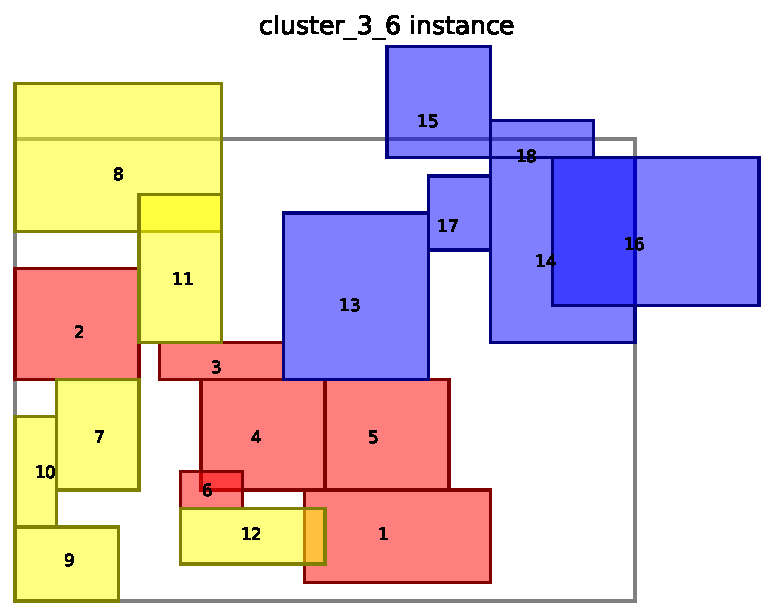
\includegraphics[width=0.49\textwidth]{visualizations/visualization_cluster_3_6}
\end{frame}

\begin{frame}{Výsledky 2/2}
	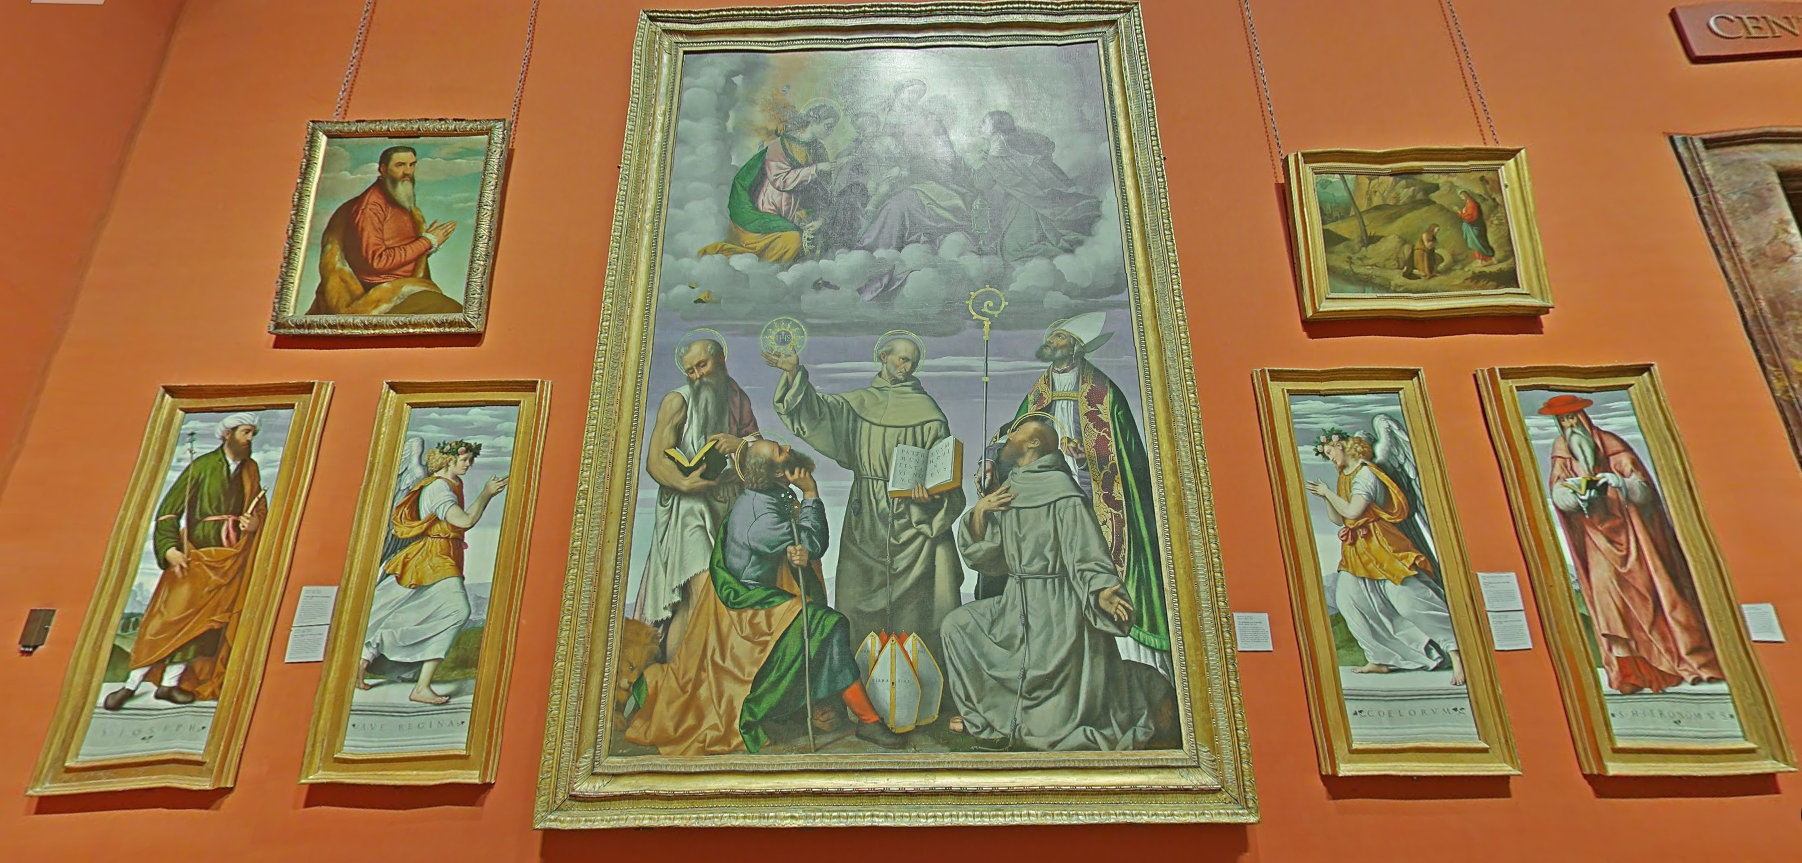
\includegraphics[width=0.49\textwidth]{london_gallery_wall}
	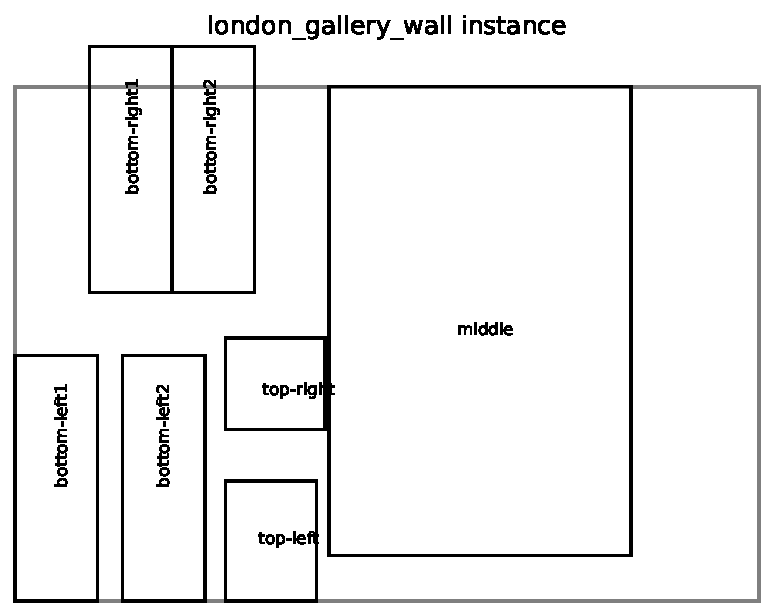
\includegraphics[width=0.49\textwidth]{visualizations/visualization_london_gallery_wall}
\end{frame}

%%%%%%%%%%%%%%%%%%%%%%%%%%%%%%%%%%%%%%%%%%%%%%%%%%%%%%%%%%%%%%%%%%%%%%%%%%%%%%
\section{Rozříšení, zlepšení, aplikace}
%%%%%%%%%%%%%%%%%%%%%%%%%%%%%%%%%%%%%%%%%%%%%%%%%%%%%%%%%%%%%%%%%%%%%%%%%%%%%%

\begin{frame}{Rozříšení, zlepšení, aplikace v jiných doménách}
	\begin{columns}[T]
		\begin{column}{.6\textwidth}
			\centering
			\begin{itemize}
				\item přidání vycpávkových (dummy) obrazů
				\item post-optimalizace
				      \begin{itemize}
					      \item přeuspořádání obrazů pro více volného místa, nepřekrývání, ...
				      \end{itemize}

				\item použití kódování pro jiné problémy
				      \begin{itemize}
					      \item knapsack, facility layout planning, ...
				      \end{itemize}

			\end{itemize}
		\end{column}

		\begin{column}{.5\textwidth}
			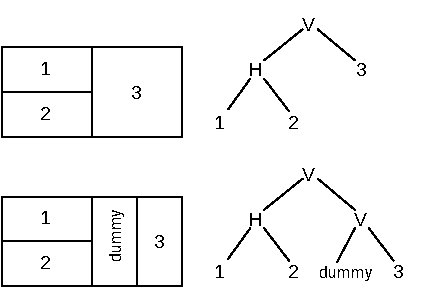
\includegraphics[width=0.8\textwidth]{dummy_painting}
		\end{column}
	\end{columns}
\end{frame}

%%%%%%%%%%%%%%%%%%%%%%%%%%%%%%%%%%%%%%%%%%%%%%%%%%%%%%%%%%%%%%%%%%%%%%%%%%%%%%
\section{Závěr}
%%%%%%%%%%%%%%%%%%%%%%%%%%%%%%%%%%%%%%%%%%%%%%%%%%%%%%%%%%%%%%%%%%%%%%%%%%%%%%

\begin{frame}
	\begin{center}
		{\fontsize{25}{35}\selectfont DĚKUJI ZA POZORNOST!\\ \vfill DOTAZY?}
	\end{center}
	\gradient{}
	\begin{itemize}
		\item cíle práce
		      \begin{itemize}
			      \item navrhnout a implementovat evoluční algoritmus pro rozmístění obrazů na stěně
			      \item vyhodnotit a vizualizovat výsledky
			      \item navrhnout zlepšení, rozšíření
		      \end{itemize}
		\item výstup
		      \begin{itemize}
			      \item představení unikátního kódování jedince a operátoru křížení
			      \item rozšíření literatury o typ řezu \textit{*}
			      \item implementace řešení, vyhodnocení výsledků a navržení rozšíření, zlepšení a aplikace v jiných doménách
		      \end{itemize}
	\end{itemize}
\end{frame}


%%%%%%%%%%%%%%%%%%%%%%%%%%%%%%%%%%%%%%%%%%%%%%%%%%%%%%%%%%%%%%%%%%%%%%%%%%%%%%%
%\section{Poděkování}
%%%%%%%%%%%%%%%%%%%%%%%%%%%%%%%%%%%%%%%%%%%%%%%%%%%%%%%%%%%%%%%%%%%%%%%%%%%%%%%
%
%\begin{frame}%%     2
%	\begin{center}
%		{\fontsize{25}{35}\selectfont DĚKUJI ZA POZORNOST!\\ \vfill DOTAZY?}
%	\end{center}
%\end{frame}

%%%%%%%%%%%%%%%%%%%%%%%%%%%%%%%%%%%%%%%%%%%%%%%%%%%%%%%%%%%%%%%%%%%%%%%%%%%%%%
% OTAZKY OPONENTA
%%%%%%%%%%%%%%%%%%%%%%%%%%%%%%%%%%%%%%%%%%%%%%%%%%%%%%%%%%%%%%%%%%%%%%%%%%%%%%

%všimněte si, že slajdy s otázky oponenta už nezvyšují číslování (jsou vlastně skryté -- odhalíte je, až na ně přijde řada; prezentaci ale zakončíte na předchozím slajdu Shrnutí).
\begin{frame}[noframenumbering]{Otázky oponenta}
	Otázka první: Proč má práce ambici zabývat se výtvarným uměním?

	\vspace{5pt}

	%	\vfill

	Otázka druhá: Navštěvuje uchazeč galerie? Pokud ano, jaké?


\end{frame}

\end{document}
